\documentclass[11pt,a4paper]{article}

\usepackage{amsfonts,amssymb,amsmath}
\usepackage[margin=1in]{geometry}
\usepackage[none]{hyphenat}
\usepackage{graphicx}
\usepackage{fancyhdr}
\usepackage{float}
\usepackage{color}
\usepackage{xcolor}
\usepackage{tikz}
\usepackage[nottoc,notlot,notlof]{tocbibind}

\usetikzlibrary{arrows.meta,patterns,shapes}

\parindent 0ex
\setlength{\parskip}{0.55\baselineskip}
\setlength{\abovedisplayskip}{0.5\baselineskip}
\setlength{\belowdisplayskip}{0.5\baselineskip}
\setlength{\abovedisplayshortskip}{0.25\baselineskip}
\setlength{\belowdisplayshortskip}{0.25\baselineskip}
\numberwithin{equation}{section}

\pagestyle{fancy}
\fancyfoot[C]{\thepage}
\fancyhead{}
\fancyhead[R]{\rightmark}
\renewcommand{\headrulewidth}{0pt}

% Upright operator names; plain italic would read Var as the product V.a.r.
\DeclareMathOperator{\Var}{Var}
\DeclareMathOperator{\Cov}{Cov}

% Theorem environments.
\usepackage{amsthm}
\theoremstyle{definition}
% One shared counter running section.subsection.n, as in the other courses here.
\newtheorem{thm}{Theorem}[subsection]
\newtheorem{defn}[thm]{Definition}
\newtheorem{exa}[thm]{Example}
\newtheorem{prop}[thm]{Proposition}
\newtheorem{coro}[thm]{Corollary}
\newtheorem{lem}[thm]{Lemma}
\newtheorem{result}[thm]{Result}
\newtheorem{exe}[thm]{Exercise}
\newtheorem*{note}{Note}
\newtheorem*{remark}{Remark}
\newtheorem{problemx}{Problem}[subsection]
\newenvironment{problem}{\begin{problemx}}{\end{problemx}}
\newenvironment{solution}
  {\renewcommand{\qedsymbol}{}\begin{proof}[\textit{Solution}.]}
  {\end{proof}}
\usepackage{enumitem}
% A heading that is legal inside a theorem body, a list or a float, where
% \subsubsection is not. Same weight as \subsubsection* so the two read alike.
\newcommand{\subhead}[1]{%
  \par\medskip\noindent\textbf{#1}\par\nobreak\smallskip}

\begin{document}
% Title page depersonalised for the web, as with every other course here. The
% identity kept below is the partition of the total sum of squares, which every
% analysis in the course is a version of.
\begin{titlepage}
\thispagestyle{empty}
\begin{center}
\vspace*{3cm}
{\Huge\bfseries Design and Analysis of Experiments}\\[1.2cm]
{\large Lecture Notes}\\[2.5cm]
\line(1,0){300}\\[1.5cm]
$$\sum_{i}\sum_{j}(y_{ij}-\bar y_{\cdot\cdot})^2 = r\sum_{i}(\bar y_{i\cdot}-\bar y_{\cdot\cdot})^2 + \sum_{i}\sum_{j}(y_{ij}-\bar y_{i\cdot})^2$$
\end{center}
\end{titlepage}

\tableofcontents
\thispagestyle{empty}
\clearpage
\setcounter{page}{1}

\section{Introduction}
An \textbf{experiment} is a test or series of tests in which changes are made to the input variables of a process or system so that the
reasons for changes in the output response may be observed and identified.

The process may be a chemical reaction, a crop growing in a field, a patient responding to a drug or a machine producing parts. In each case
some inputs are under the experimenter's control, some are not, and the output is affected by both (Figure~\ref{fig:process}).

% The stub of the original notes left "% diagram" at this point. This is the
% standard picture of a process: controllable inputs from above, uncontrollable
% ones from below, and the response that depends on both.
\begin{figure}[H]
\centering
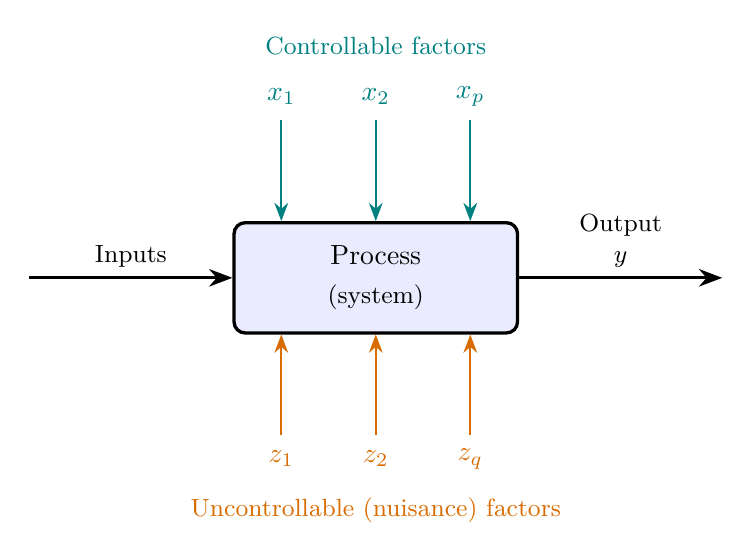
\begin{tikzpicture}[scale=1,
  box/.style={draw,very thick,rounded corners=4pt,fill=blue!8,minimum width=3.6cm,minimum height=1.4cm,align=center},
  lab/.style={font=\small,align=center}]
\node[box] (P) at (0,0) {Process\\[2pt]\small(system)};
\draw[-Stealth,very thick] (-4.4,0) -- (P.west) node[midway,above,lab] {Inputs};
\draw[-Stealth,very thick] (P.east) -- (4.4,0) node[midway,above,lab] {Output\\$y$};
\foreach \x/\l in {-1.2/x_1,0/x_2,1.2/x_p} {
  \draw[-Stealth,thick,teal] (\x,2.0) -- (\x,0.72);
  \node[teal] at (\x,2.3) {$\l$};
}
\node[teal,lab] at (0,2.95) {Controllable factors};
\foreach \x/\l in {-1.2/z_1,0/z_2,1.2/z_q} {
  \draw[-Stealth,thick,orange!85!black] (\x,-2.0) -- (\x,-0.72);
  \node[orange!85!black] at (\x,-2.3) {$\l$};
}
\node[orange!85!black,lab] at (0,-2.95) {Uncontrollable (nuisance) factors};
\end{tikzpicture}
\caption{A general model of a process. The experimenter sets the controllable factors $x_1,\dots,x_p$; the factors $z_1,\dots,z_q$
also affect the response $y$ but are not set by the experimenter.}
\label{fig:process}
\end{figure}

The objectives of an experiment may include determining which factors have the most influence on the response, where to set the
controllable factors so that the response is near a target, or so that its variability is small, and where to set them so that the effects of the
uncontrollable factors are minimised.

\textbf{Statistical design of experiments} refers to the process of planning the experiment so that appropriate data that can be analysed by
statistical methods will be collected, resulting in valid and objective conclusions.

Design and analysis cannot be separated. The design decides which comparisons the data can support and with what precision; the analysis
can only extract what the design has put there. A well-designed experiment is often analysed with nothing more than a table of means. A badly
designed one cannot be rescued by any analysis, however sophisticated. R.~A.~Fisher put it bluntly: to consult the statistician after an
experiment is finished is often merely to ask him to conduct a post mortem examination; he can perhaps say what the experiment died of.

\subsection{Basic terminology}
\begin{defn}
\begin{enumerate}[label=(\roman*)]
\item A \textbf{factor} is an input variable whose effect on the response is studied. Its chosen values are its \textbf{levels}. A factor may be
\textbf{quantitative} (temperature: $150$, $160$, $170\,^\circ$C) or \textbf{qualitative} (brand of tyre: $A$, $B$).
\item A \textbf{treatment} is the combination of factor levels applied to a unit. With one factor the treatments are its levels; with several
they are the combinations of their levels.
\item An \textbf{experimental unit} is the smallest piece of material to which a treatment is applied independently of the others: a plot of land, an animal,
a batch of raw material, a run of a machine.
\item A \textbf{measurement unit} (or observational unit) is the object on which the response is measured. It may be the experimental unit
or a part of it.
\item The \textbf{response} is the variable measured to assess the effect of the treatments.
\item \textbf{Experimental error} is the variation among experimental units that receive the same treatment.
\end{enumerate}
\end{defn}

The distinction between experimental and measurement units matters more than any other in this course, because experimental error, and
so every test and confidence interval, must be measured between experimental units.

\begin{exa}\label{exa:pens}
Two diets are compared on pigs. Eight pens hold five pigs each; four pens are chosen at random to receive diet $1$ and the other four diet $2$,
and every pig is weighed after six weeks. The diet is applied to a whole pen, so the experimental unit is the \emph{pen}, and there are four
replicates of each diet, not twenty. The pigs are measurement units. Pigs in the same pen share a trough, a draught and a pen-mate who
bullies them, so their weights are correlated; treating the $40$ weights as $40$ independent replicates understates the experimental error and
overstates the evidence. This mistake is called \textbf{pseudo-replication}.
\end{exa}

\subsection{Principles of experimental design}
Three principles underlie every design in this course.

\begin{defn}
\begin{enumerate}[label=(\roman*)]
\item \textbf{Replication} is the repetition of the basic experiment: each treatment is applied independently to more than one experimental
unit.
\item \textbf{Randomisation} is the use of a chance mechanism to allocate the treatments to the experimental units, and to fix the order in
which the individual runs of the experiment are performed.
\item \textbf{Blocking} is the grouping of experimental units into sets (blocks) that are more alike than the units as a whole, and the
comparison of treatments within the blocks. Equivalently, it fixes the levels of a nuisance factor while the factors of interest are varied.
\end{enumerate}
\end{defn}

Each principle has two jobs.

\subhead{Replication}
\begin{itemize}
\item It allows the experimenter to obtain an estimate of the experimental error, which is the yardstick against which differences between
treatments are judged. Without replication there is no way to tell a treatment difference from unit-to-unit variation.
\item It makes the estimates more precise: if $\sigma^2$ is the variance of a single observation, the mean of $r$ replicates has variance
$\sigma^2/r$.
\end{itemize}
Replication is not the same as repeated measurement. Weighing the same pig three times reduces measurement error but tells us nothing about
variation between pigs.

\subhead{Randomisation}
\begin{itemize}
\item It makes valid the assumption, required by the statistical methods, that the observations (or errors) are independently distributed
random variables.
\item It helps average out the effects of factors that are unknown or not controlled, so that no treatment is systematically favoured.
\end{itemize}

\subhead{Blocking}
\begin{itemize}
\item It improves the precision of comparisons between the factors of interest.
\item It reduces or eliminates the effect of known nuisance factors on those comparisons.
\end{itemize}

The rule that follows is short: \emph{block what you can, randomise what you cannot}.

\subsection{Randomisation as the basis of inference}
The claim that randomisation ``validates'' the analysis can be made precise. Suppose $N = 2n$ experimental units are available and
two treatments $A$ and $B$ are to be compared. Assume \textbf{unit--treatment additivity}: unit $k$ would give response
\[
y_k = u_k + \tau_A \quad\text{under } A , \qquad y_k = u_k + \tau_B \quad\text{under } B ,
\]
where $u_k$ is a fixed but unknown unit value and $\tau_A$, $\tau_B$ are the treatment effects. Nothing is assumed about the $u_k$: they need not
be normal, independent or even random. Write
\[
\bar u = \frac1N\sum_{k=1}^Nu_k , \qquad S^2 = \frac{1}{N - 1}\sum_{k=1}^N(u_k - \bar u)^2 .
\]
In a \textbf{completely randomised} allocation, a set of $n$ units is chosen at random, every one of the $\binom Nn$ sets being equally likely,
and these receive $A$; the rest receive $B$. The only randomness is in the allocation.

\begin{lem}\label{lem:srswor}
Let $\bar u_A$ be the mean of the unit values in a random set of $n$ of the $N$ units. Then
\[
E(\bar u_A) = \bar u , \qquad \Var(\bar u_A) = \frac{S^2}{n}\Bigl(1 - \frac nN\Bigr) .
\]
\end{lem}

\begin{proof}
Let $I_k = 1$ if unit $k$ is in the set and $0$ otherwise, so $\bar u_A = \frac1n\sum_kI_ku_k$. By symmetry $P(I_k = 1) = n/N$ for every $k$, and for
$k \ne l$, $P(I_k = I_l = 1) = \frac{n(n - 1)}{N(N - 1)}$. Hence $E(\bar u_A) = \frac1n\sum_k\frac nNu_k = \bar u$, and
\begin{gather*}
\Var(I_k) = \frac nN\Bigl(1 - \frac nN\Bigr) , \\
\Cov(I_k, I_l) = \frac{n(n - 1)}{N(N - 1)} - \frac{n^2}{N^2} = -\frac{n(N - n)}{N^2(N - 1)} .
\end{gather*}
Since $\bar u_A - \bar u = \frac1n\sum_kI_k(u_k - \bar u)$ and $\sum_k(u_k - \bar u) = 0$, write $v_k = u_k - \bar u$. Then
\begin{align*}
n^2\Var(\bar u_A) &= \sum_kv_k^2\Var(I_k) + \sum_{k\ne l}v_kv_l\Cov(I_k, I_l) \\
&= \frac{n(N - n)}{N^2}\Bigl[\sum_kv_k^2 - \frac{1}{N - 1}\sum_{k\ne l}v_kv_l\Bigr] .
\end{align*}
Since $\sum_{k\ne l}v_kv_l = \bigl(\sum_kv_k\bigr)^2 - \sum_kv_k^2 = -\sum_kv_k^2$, the term in brackets is $\sum_kv_k^2\bigl(1 + \frac{1}{N - 1}\bigr) = \frac{N}{N - 1}\sum_kv_k^2 = NS^2$. So
\[
\Var(\bar u_A) = \frac{N - n}{nN}S^2 = \frac{S^2}{n}\Bigl(1 - \frac nN\Bigr) .
\]
\end{proof}

\begin{thm}\label{thm:randomisation}
Under unit--treatment additivity and complete randomisation of $2n$ units, $n$ to each treatment, the difference of treatment means satisfies
\[
E(\bar y_A - \bar y_B) = \tau_A - \tau_B , \qquad \Var(\bar y_A - \bar y_B) = \frac{2S^2}{n} .
\]
\end{thm}

\begin{proof}
$\bar y_A - \bar y_B = \tau_A - \tau_B + \bar u_A - \bar u_B$, and since the two groups together contain every unit, $n\bar u_A + n\bar u_B = N\bar u$, that
is $\bar u_B = 2\bar u - \bar u_A$. Hence $\bar u_A - \bar u_B = 2(\bar u_A - \bar u)$, which has mean $0$ and, by Lemma~\ref{lem:srswor} with $N = 2n$,
variance $4\cdot\frac{S^2}{n}\cdot\frac12 = 2S^2/n$.
\end{proof}

\begin{remark}
Compare Theorem~\ref{thm:randomisation} with the familiar result for independent observations with variance $\sigma^2$, namely
$\Var(\bar Y_A - \bar Y_B) = 2\sigma^2/n$. The formulas coincide with $S^2$ in place of $\sigma^2$, but the randomisation version assumes nothing about
the units: the probability comes from the coin the experimenter tossed, not from a model of nature. This is the precise sense in which
randomisation justifies the analysis. Without it, a systematic allocation (say the $n$ units nearest the door to $A$) could make $\bar u_A - \bar u_B$
anything at all, and no amount of data would reveal the bias.
\end{remark}

\begin{exa}\label{exa:randomisation-dist}
Eight units have values $u = (3, 7, 1, 9, 4, 4, 8, 2)$, so $\bar u = 4.75$ and $S^2 = 8.5$. There are $\binom84 = 70$ ways to choose the four units
for $A$. Taking $\tau_A = \tau_B$ and listing all $70$ values of $\bar u_A - \bar u_B$ gives a distribution with mean exactly $0$ and variance
exactly $4.25 = 2S^2/n$, as Theorem~\ref{thm:randomisation} says. This \textbf{randomisation distribution} is also the basis of an exact test: an
observed difference is significant at level $\alpha$ if it lies in the extreme $100\alpha\%$ of the $70$ values.
\end{exa}

\subsection{Blocking: the tyre example}
\begin{exa}\label{exa:tyres}
Suppose we want to compare two brands of tyres, $A$ and $B$, by the tread wear after a fixed distance. Possible complicating factors include
\begin{enumerate}[label=(\roman*)]
\item the type of car;
\item road conditions;
\item the type of driver;
\end{enumerate}
and so on. How do we control for them? Known factors are handled by blocking, and unknown ones by randomisation. Consider the possible
experimental strategies.

\begin{enumerate}[label=(\alph*)]
\item \textbf{$2n$ cars.} Choose $n$ cars at random for brand $A$ and fit the other $n$ with brand $B$. Then $\mu_A - \mu_B$ is estimated by
$\bar y_A - \bar y_B$, with
\[
E(\bar Y_A - \bar Y_B) = \mu_A - \mu_B , \qquad \Var(\bar Y_A - \bar Y_B) = \frac{2\sigma^2}{n} ,
\]
where $\sigma^2$ is the variance of the wear on a single car. The only way to reduce this variance is to increase $n$.

\item \textbf{$n$ good drivers and $n$ rough drivers.} There are now two possible strategies.
\begin{enumerate}[label=(\roman*)]
\item Randomly assign $n$ of the $2n$ drivers to brand $A$ and the other $n$ to brand $B$, ignoring the type of driver. The variance $\sigma_1^2$ of
$\bar y_A - \bar y_B$ then includes variation between brands and among drivers.
\item Randomly assign half ($n/2$) of the good drivers to brand $A$ and the other half to brand $B$, and do the same for the rough drivers.
Writing $\bar y_{1A}$ for the mean of the good drivers on brand $A$, and so on, estimate $\mu_A - \mu_B$ by
\[
\frac{\bar y_{1A} + \bar y_{2A} - (\bar y_{1B} + \bar y_{2B})}{2} ,
\]
with variance $\sigma_2^2$.
\end{enumerate}
The second strategy gives the higher precision, $\sigma_2^2 < \sigma_1^2$. Proposition~\ref{prop:drivers} below says by how much.

\item \textbf{$n$ cars, both brands on each.} Fit brand $A$ on one side of each car and brand $B$ on the other, choosing the side at random. The
car is now a block of two units, and each car gives a difference $d_k = y_{kA} - y_{kB}$ in which the car's own effect cancels.
\end{enumerate}
\end{exa}

To compare the strategies we need a model for the wear. Write the wear of a tyre of brand $T$ on car (or driver) $k$ as
\[
y = \mu_T + \beta_k + \varepsilon ,
\]
where $\beta_k$ is the effect of the car or driver and $\varepsilon$, with variance $\sigma^2$, is the remaining variation of a tyre about its car's level.

\begin{prop}\label{prop:drivers}
In strategy (b), let good drivers have $\beta = -\delta$ and rough drivers $\beta = +\delta$, and let the errors be independent with variance $\sigma^2$. Then
\[
\sigma_1^2 = \frac{2\sigma^2}{n} + \frac{4\delta^2}{2n - 1} , \qquad \sigma_2^2 = \frac{2\sigma^2}{n} .
\]
\end{prop}

\begin{proof}
For (i), apply Theorem~\ref{thm:randomisation} conditionally on the errors, with unit values $u_k = \beta_k + \varepsilon_k$. The driver effects
are $n$ values $-\delta$ and $n$ values $+\delta$, with mean $0$ and $\sum\beta_k^2 = 2n\delta^2$, so taking expectations over the errors,
\[
E(S^2) = \sigma^2 + \frac{2n\delta^2}{2n - 1} , \qquad\text{and}\qquad \sigma_1^2 = \frac2nE(S^2) = \frac{2\sigma^2}{n} + \frac{4\delta^2}{2n - 1} .
\]
For (ii), each of the four group means is over $n/2$ drivers of the same type. In $\bar y_{1A} - \bar y_{1B}$ the good drivers' $-\delta$ cancels, and in
$\bar y_{2A} - \bar y_{2B}$ the rough drivers' $+\delta$ cancels, so only the errors remain:
\[
\sigma_2^2 = \frac14\cdot4\cdot\frac{\sigma^2}{n/2} = \frac{2\sigma^2}{n} .
\]
\end{proof}

The driver effect has not been reduced by strategy (ii); it has been removed from the comparison entirely, by balancing it across the brands.
Strategy (c) goes further. Each $d_k = \mu_A - \mu_B + \varepsilon_{kA} - \varepsilon_{kB}$ is free of every car effect, known or unknown, so with $n$ cars
\[
\Var(\bar d) = \frac{2\sigma^2}{n} .
\]
In strategy (a), on the other hand, the car-to-car variation $\sigma_\beta^2$ enters each observation, and $\Var(\bar y_A - \bar y_B) = 2(\sigma_\beta^2 + \sigma^2)/n$
with $2n$ cars. Blocking on cars therefore gives the same number of comparisons from half the cars, with the variance reduced by the factor
$\sigma^2/(\sigma_\beta^2 + \sigma^2)$. When cars differ a great deal, which in a wear study they do, the gain is large. Strategy (c) is the
\textbf{paired comparison} design of the next section, the simplest case of the randomised block design.

\subsection{Strategies of experimentation}
\begin{exa}\label{exa:football}
The performance of a football team depends on many factors. Some of them may be
\begin{enumerate}[label=(\alph*)]
\item the coach (local or expatriate);
\item the type of boot (metal or plastic studs);
\item the time of playing (afternoon or night);
\item the type of ball (ordinary or designer);
\end{enumerate}
and so on. How do we find the combination that gives the best performance?
\end{exa}

There are three broad strategies.

\begin{enumerate}[label=(\roman*)]
\item \textbf{Best-guess approach.} Select an arbitrary combination of the factors, test it and see what happens. Then change the levels of one or
two factors, guided by experience, and test again, and so on. This often works reasonably well when the experimenter knows the system
well, but there is no guarantee of success, and no way of knowing when to stop or whether the best combination has been found.
\item \textbf{One-factor-at-a-time (OFAT) approach.} Select a starting point, or baseline set of levels, for each factor. Then successively vary each
factor over its range with the other factors held constant at the baseline levels. The results are summarised in a series of graphs, each
showing how the response is affected by varying one factor with all the others held constant.
\item \textbf{Factorial experiment.} The factors are varied \emph{together} instead of one at a time: the runs consist of all (or a chosen subset of)
the combinations of the levels of the factors.
\end{enumerate}

% Infographic in the style the user asked for: one panel per strategy, each
% showing which points of the coach x ball square are actually run.
\begin{figure}[H]
\centering
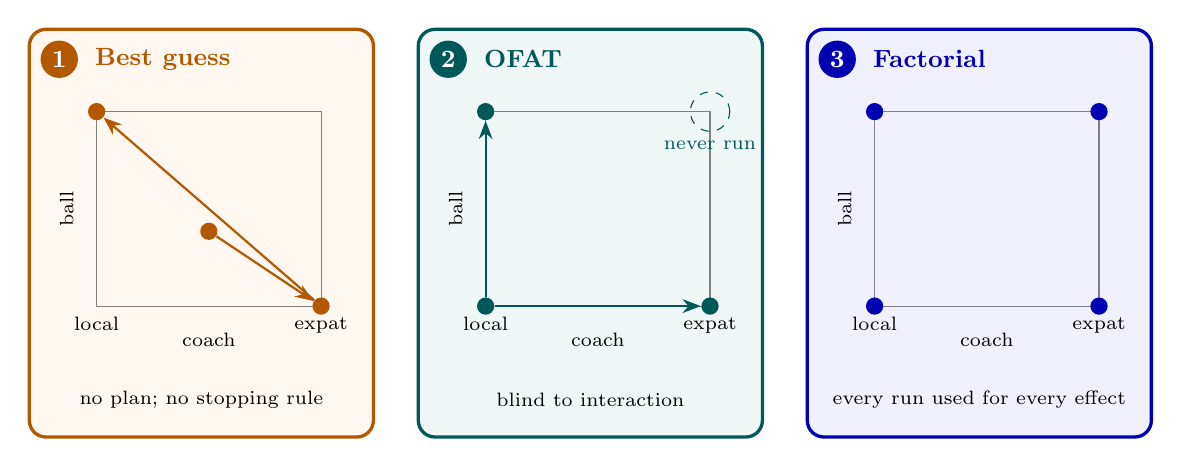
\begin{tikzpicture}[scale=0.95,
  pt/.style={circle,fill,inner sep=2.2pt},
  panel/.style={rounded corners=6pt,very thick}]
% panel frames
\foreach \x/\c/\n/\t in {0/orange/1/Best guess,5.2/teal/2/OFAT,10.4/blue/3/Factorial} {
  \draw[panel,draw=\c!70!black,fill=\c!6] (\x-0.3,-1.35) rectangle (\x+4.3,4.1);
  \node[circle,fill=\c!70!black,text=white,font=\bfseries\small,inner sep=2pt] at (\x+0.1,3.7) {\n};
  \node[font=\bfseries\small,\c!70!black,anchor=west] at (\x+0.45,3.7) {\t};
  % the factor square
  \draw[gray] (\x+0.6,0.4) rectangle (\x+3.6,3.0);
  \node[font=\scriptsize] at (\x+2.1,-0.05) {coach};
  \node[font=\scriptsize,rotate=90] at (\x+0.2,1.7) {ball};
  \node[font=\scriptsize,anchor=north] at (\x+0.6,0.38) {local};
  \node[font=\scriptsize,anchor=north] at (\x+3.6,0.38) {expat};
}
% 1: a wandering path of guesses
\node[pt,orange!70!black] (g1) at (2.1,1.4) {};
\node[pt,orange!70!black] (g2) at (3.6,0.4) {};
\node[pt,orange!70!black] (g3) at (0.6,3.0) {};
\draw[-Stealth,orange!70!black,thick] (g1) -- (g2);
\draw[-Stealth,orange!70!black,thick] (g2) -- (g3);
\node[font=\scriptsize,align=center] at (2.0,-0.85) {no plan; no stopping rule};
% 2: baseline, then one factor moved at a time
\node[pt,teal!70!black] (o0) at (5.8,0.4) {};
\node[pt,teal!70!black] (o1) at (8.8,0.4) {};
\node[pt,teal!70!black] (o2) at (5.8,3.0) {};
\draw[-Stealth,teal!70!black,thick] (o0) -- (o1);
\draw[-Stealth,teal!70!black,thick] (o0) -- (o2);
\node[draw,teal!70!black,dashed,circle,minimum size=0.5cm] at (8.8,3.0) {};
\node[font=\scriptsize,teal!70!black] at (8.8,2.55) {never run};
\node[font=\scriptsize,align=center] at (7.2,-0.85) {blind to interaction};
% 3: all four corners
\foreach \p in {(11.0,0.4),(14.0,0.4),(11.0,3.0),(14.0,3.0)} \node[pt,blue!70!black] at \p {};
\node[font=\scriptsize,align=center] at (12.4,-0.85) {every run used for every effect};
\end{tikzpicture}
\caption{Three strategies for two factors at two levels. The OFAT experiment never visits the combination of expatriate coach and designer
ball, so it cannot tell whether the two factors act together.}
\label{fig:strategies}
\end{figure}

The weakness of the OFAT approach is that it fails to consider any possible \textbf{interaction} between the factors.

\begin{defn}
Two factors \textbf{interact} when the effect of one factor on the response is not the same at the different levels of the other factor.
\end{defn}

For two factors $A$ and $B$ at two levels each, write $\bar y_{A^-B^-}$ for the mean response with both at their low levels, and so on. The effect
of $A$ at the low level of $B$ is $\bar y_{A^+B^-} - \bar y_{A^-B^-}$, and at the high level of $B$ it is $\bar y_{A^+B^+} - \bar y_{A^-B^+}$. The \textbf{main effect} of $A$
is their average, and the \textbf{interaction} $AB$ is half their difference:
\begin{align*}
A &= \tfrac12\bigl[(\bar y_{A^+B^-} - \bar y_{A^-B^-}) + (\bar y_{A^+B^+} - \bar y_{A^-B^+})\bigr] , \\
AB &= \tfrac12\bigl[(\bar y_{A^+B^+} - \bar y_{A^-B^+}) - (\bar y_{A^+B^-} - \bar y_{A^-B^-})\bigr] .
\end{align*}
The definition of $AB$ is symmetric in $A$ and $B$: it is also half the difference between the effects of $B$ at the two levels of $A$.

\begin{exa}\label{exa:coach-ball}
In Example~\ref{exa:football}, suppose the mean goals per match for the four combinations of coach ($A$: local $-$, expatriate $+$) and ball
($B$: ordinary $-$, designer $+$) are
\begin{center}
\begin{tabular}{l|cc}
 & ordinary ball & designer ball \\
\hline
local coach & $1.0$ & $0.8$ \\
expatriate coach & $0.9$ & $1.6$
\end{tabular}
\end{center}
The effect of the coach is $0.9 - 1.0 = -0.1$ with the ordinary ball but $1.6 - 0.8 = +0.8$ with the designer ball, so
\[
A = \tfrac12(-0.1 + 0.8) = 0.35 , \qquad AB = \tfrac12\bigl(0.8 - (-0.1)\bigr) = 0.45 .
\]
The interaction is larger than the main effect: the expatriate coach is worth having only with the designer ball (Figure~\ref{fig:interaction}).

Now suppose the team ran an OFAT experiment from the baseline (local coach, ordinary ball), at $1.0$ goals. Changing the coach gives $0.9$, worse, so
the local coach is kept; changing the ball then gives $0.8$, worse again, so the ordinary ball is kept. The OFAT experiment concludes that the
baseline is best, and never discovers the combination that gives $1.6$.
\end{exa}

\begin{figure}[H]
\centering
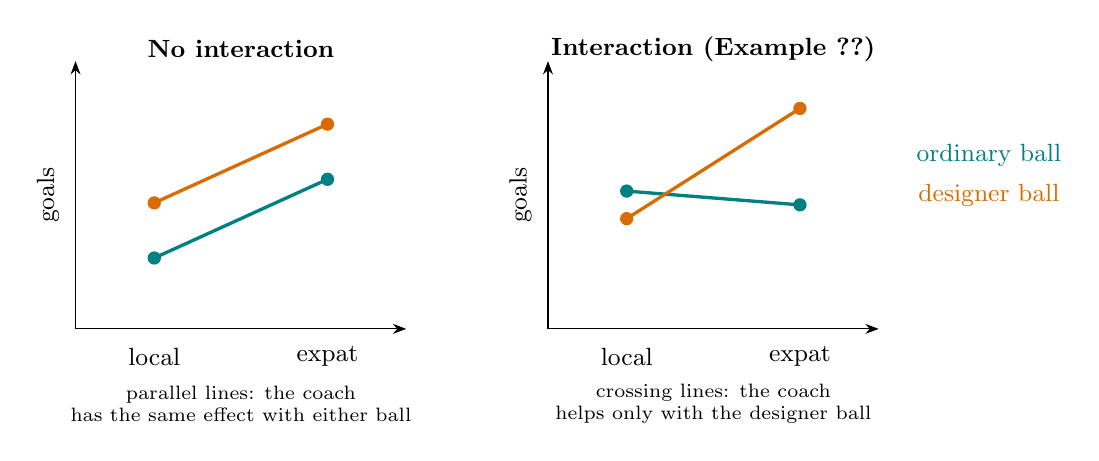
\begin{tikzpicture}[scale=1]
% left panel: no interaction
\begin{scope}
\draw[-Stealth] (0,0) -- (4.2,0);
\draw[-Stealth] (0,0) -- (0,3.4);
\node[rotate=90,font=\small] at (-0.35,1.7) {goals};
\node[font=\small] at (1,-0.35) {local}; \node[font=\small] at (3.2,-0.35) {expat};
\draw[very thick,teal] (1,0.9) -- (3.2,1.9);
\draw[very thick,orange!85!black] (1,1.6) -- (3.2,2.6);
\foreach \p in {(1,0.9),(3.2,1.9)} \fill[teal] \p circle (2.4pt);
\foreach \p in {(1,1.6),(3.2,2.6)} \fill[orange!85!black] \p circle (2.4pt);
\node[font=\small\bfseries] at (2.1,3.55) {No interaction};
\node[font=\scriptsize,align=center] at (2.1,-0.95) {parallel lines: the coach\\has the same effect with either ball};
\end{scope}
% right panel: the data of the example
\begin{scope}[xshift=6cm]
\draw[-Stealth] (0,0) -- (4.2,0);
\draw[-Stealth] (0,0) -- (0,3.4);
\node[rotate=90,font=\small] at (-0.35,1.7) {goals};
\node[font=\small] at (1,-0.35) {local}; \node[font=\small] at (3.2,-0.35) {expat};
% scale 1 goal = 1.75 units
\draw[very thick,teal] (1,1.75) -- (3.2,1.575);
\draw[very thick,orange!85!black] (1,1.40) -- (3.2,2.80);
\foreach \p in {(1,1.75),(3.2,1.575)} \fill[teal] \p circle (2.4pt);
\foreach \p in {(1,1.40),(3.2,2.80)} \fill[orange!85!black] \p circle (2.4pt);
\node[font=\small\bfseries] at (2.1,3.55) {Interaction (Example~\ref{exa:coach-ball})};
\node[font=\scriptsize,align=center] at (2.1,-0.95) {crossing lines: the coach\\helps only with the designer ball};
\end{scope}
\node[teal,font=\small] at (11.6,2.2) {ordinary ball};
\node[orange!85!black,font=\small] at (11.6,1.7) {designer ball};
\end{tikzpicture}
\caption{Interaction plots: mean response against the level of one factor, one line for each level of the other.}
\label{fig:interaction}
\end{figure}

The factorial experiment is the correct approach for dealing with several factors. It detects interactions, and it is also more efficient, even
when there are none.

\begin{prop}\label{prop:ofat}
Suppose there are $k$ factors at two levels, no interactions, and errors with variance $\sigma^2$. An OFAT experiment that runs the baseline and the
$k$ one-factor changes, $m$ times each, estimates every main effect with variance $2\sigma^2/m$ and uses $(k + 1)m$ runs. A balanced two-level
factorial experiment achieves the same variance with $2m$ runs. The OFAT experiment therefore needs $(k + 1)/2$ times as many runs.
\end{prop}

\begin{proof}
In the OFAT experiment the effect of factor $j$ is estimated by $\bar y_j - \bar y_0$, the difference between the mean of the $m$ runs with factor $j$
changed and the mean of the $m$ baseline runs, with variance $\sigma^2/m + \sigma^2/m = 2\sigma^2/m$. In a balanced factorial with $N$ runs, half the runs
have factor $j$ high and half low, and its effect is estimated by $\bar y_{j^+} - \bar y_{j^-}$, a difference of two means of $N/2$ runs each, with
variance $2\sigma^2/(N/2) = 4\sigma^2/N$. This equals $2\sigma^2/m$ when $N = 2m$. The ratio of run counts is $(k + 1)m/(2m) = (k + 1)/2$.
\end{proof}

The source of the saving is sometimes called \textbf{hidden replication}: in a factorial experiment every run contributes to the estimate of every
main effect, whereas in an OFAT experiment each run contributes to the estimates of at most two. With $k = 2$ factors the factorial needs two thirds
of the runs; with $k = 7$ it needs a quarter. (A full $2^k$ factorial has $2^k$ runs, which can be more than $2m$; the fractional factorials of a later
section remove that restriction.)

\subsection{Guidelines for designing an experiment}
\begin{enumerate}
\item \textbf{Recognition and statement of the problem.} Write down the objectives. A clear statement often makes the design obvious; a vague one
guarantees an experiment that answers nothing in particular.
\item \textbf{Choice of factors, levels and ranges.} Distinguish the design factors from the nuisance factors, and decide how each nuisance factor is to
be handled: blocked if it can be controlled, measured and adjusted for if it can only be observed, randomised over if it is unknown.
\item \textbf{Selection of the response variable.} It should measure what the objectives are about, and be measurable with known precision.
\item \textbf{Choice of experimental design.} This includes the number of replicates, the run order and any blocking, and should be made with the
analysis in mind.
\item \textbf{Performing the experiment.} Monitor the process to make sure everything is done according to plan; errors in procedure at this
stage usually destroy the validity of the experiment.
\item \textbf{Statistical analysis of the data.} Estimates, tests and confidence intervals, together with residual checks of the model's
assumptions.
\item \textbf{Conclusions and recommendations.} Practical conclusions, followed where necessary by confirmation runs.
\end{enumerate}
Steps 1--3 are often called \textbf{pre-experimental planning}. Experimentation is also sequential: a first small screening experiment identifies
the important factors, and later experiments study those factors in more detail.

\subsection{A short history}
The statistical design of experiments was created by R.~A.~Fisher at the Rothamsted agricultural research station in England in the 1920s.
Faced with decades of field records from which little could be learned, he introduced randomisation, replication and blocking, the analysis of
variance and factorial designs, and set them out in \emph{The Design of Experiments} (1935). F.~Yates extended the work to confounding and
incomplete blocks. In the 1950s G.~E.~P.~Box and K.~B.~Wilson brought the ideas into the chemical industry with response surface methodology,
where experiments are run in sequence and the results are available quickly. From the 1980s the work of G.~Taguchi on robust design,
experiments that make a product insensitive to uncontrollable factors, spread the methods through manufacturing. The principles have not
changed since Fisher; the applications now run from agriculture and medicine to engineering and computer simulation.

\subsection{Practice problems}

\begin{problem}
State and define the three principles of experimental design, and give one reason why each is important.
\end{problem}

\begin{solution}
\emph{Replication}: each treatment is applied independently to several experimental units; it provides an estimate of the experimental
error, without which treatment differences cannot be judged. \emph{Randomisation} is the use of a chance mechanism to allocate treatments to units and
to order the runs; it makes the errors behave as independent random variables and protects against bias from uncontrolled factors.
\emph{Blocking} is the grouping of similar units into blocks within which the treatments are compared; it removes the effect of a known nuisance
factor from the comparisons and so increases their precision.
\end{solution}

\begin{problem}
Four fields are available. Two are chosen at random to be irrigated and two are not. Each field is divided into six plots, and three fertilisers are
allocated at random to the plots within each field, two plots each. The yield of every plot is recorded. Identify the experimental unit for
irrigation and for fertiliser, and the number of replicates of each irrigation level.
\end{problem}

\begin{solution}
Irrigation is applied to whole fields, so the field is the experimental unit for irrigation, and each irrigation level has only two replicates, however
many plots are measured. Fertiliser is applied to plots, so the plot is the experimental unit for fertiliser. The two factors have different
experimental units and so different experimental errors; this is a split-plot experiment, analysed in a later section. Comparing irrigation levels
against the plot-to-plot variation would be pseudo-replication.
\end{solution}

\begin{problem}
Four units have values $u = (5, 9, 6, 12)$, and two treatments with $\tau_A = \tau_B$ are allocated completely at random, two units each. List the
randomisation distribution of $\bar y_A - \bar y_B$ and verify Theorem~\ref{thm:randomisation}.
\end{problem}

\begin{solution}
Here $\bar u = 8$ and $S^2 = (9 + 1 + 4 + 16)/3 = 10$, so the theorem predicts mean $0$ and variance $2S^2/n = 10$. The $\binom42 = 6$ allocations give
\begin{center}
\begin{tabular}{cc|c}
units on $A$ & units on $B$ & $\bar y_A - \bar y_B$ \\
\hline
$5, 9$ & $6, 12$ & $-2$ \\
$5, 6$ & $9, 12$ & $-5$ \\
$5, 12$ & $9, 6$ & $1$ \\
$6, 12$ & $5, 9$ & $2$ \\
$9, 12$ & $5, 6$ & $5$ \\
$9, 6$ & $5, 12$ & $-1$
\end{tabular}
\end{center}
Each value is equally likely. The mean is $0$ and the variance is $2(4 + 25 + 1)/6 = 10$, as predicted.
\end{solution}

\begin{problem}
In a tyre wear study the variance between cars is $\sigma_\beta^2 = 3$ and the variance of a tyre about its car's level is $\sigma^2 = 1$ (in suitable
units). A completely randomised design uses $20$ cars, $10$ per brand. How many cars would a paired design (strategy (c) of
Example~\ref{exa:tyres}) need to estimate $\mu_A - \mu_B$ at least as precisely?
\end{problem}

\begin{solution}
The completely randomised design gives $\Var(\bar y_A - \bar y_B) = 2(\sigma_\beta^2 + \sigma^2)/10 = 2(4)/10 = 0.8$. The paired design with $n$ cars gives
$\Var(\bar d) = 2\sigma^2/n = 2/n$, which is at most $0.8$ when $n \ge 2.5$. Three cars suffice, against twenty. In practice more would be used, to estimate
$\sigma^2$ with reasonable precision and to check the assumptions, but the comparison shows how much blocking can save.
\end{solution}

\begin{problem}
The mean responses of a two-factor experiment are $20$ at $(A^-, B^-)$, $30$ at $(A^+, B^-)$, $40$ at $(A^-, B^+)$ and $12$ at $(A^+, B^+)$. Compute the
main effects and the interaction. An OFAT experiment starts from $(A^-, B^-)$, varies $A$ first and keeps the better level, then varies $B$. Which
combination does it recommend?
\end{problem}

\begin{solution}
The effect of $A$ is $30 - 20 = 10$ at $B^-$ and $12 - 40 = -28$ at $B^+$, so $A = \frac12(10 - 28) = -9$ and $AB = \frac12(-28 - 10) = -19$. The effect of $B$ is
$40 - 20 = 20$ at $A^-$ and $12 - 30 = -18$ at $A^+$, so $B = \frac12(20 - 18) = 1$. The main effects are small and the interaction is large: each factor's
effect reverses with the level of the other.

The OFAT experiment finds $30 > 20$ and moves to $A^+$; at $A^+$ it finds $12 < 30$ and keeps $B^-$. It recommends $(A^+, B^-)$ with response $30$, and misses
$(A^-, B^+)$ with $40$, a combination it never runs.
\end{solution}

\begin{problem}
Three factors at two levels are to be studied, and each main effect is to be estimated with variance $\sigma^2/2$. How many runs does an OFAT
experiment need, and how many does a factorial experiment need?
\end{problem}

\begin{solution}
OFAT gives variance $2\sigma^2/m$, so $m = 4$ runs at each of the $k + 1 = 4$ conditions: $16$ runs. A balanced factorial gives $4\sigma^2/N$, so $N = 8$: one
replicate of the $2^3 = 8$ combinations. The factorial uses half the runs, in agreement with Proposition~\ref{prop:ofat}, and it estimates the three
two-factor interactions as well.
\end{solution}

\section{Simple comparative experiments}
The simplest experiment compares two treatments. It is worth treating carefully, because every idea of the later sections appears here in its
plainest form: a model for the observations, an estimate of experimental error, a test and a confidence interval, a check of the assumptions,
a choice of sample size, and the gain from blocking.

\begin{exa}\label{exa:catalyst}
A chemical engineer compares the yield (\%) of a process run with two catalysts. Sixteen batches of raw material are available; eight are
chosen at random for catalyst $A$ and the other eight are run with catalyst $B$, in random order. The yields are
\begin{center}
\begin{tabular}{c|cc}
batch & catalyst $A$ & catalyst $B$ \\
\hline
$1$ & $91.5$ & $89.2$ \\
$2$ & $94.2$ & $91.0$ \\
$3$ & $92.2$ & $90.5$ \\
$4$ & $95.4$ & $93.2$ \\
$5$ & $91.8$ & $88.9$ \\
$6$ & $89.1$ & $87.6$ \\
$7$ & $94.7$ & $90.1$ \\
$8$ & $89.2$ & $89.9$ \\
\hline
$\bar y_i$ & $92.2625$ & $90.0500$ \\
$s_i^2$ & $5.6741$ & $2.7286$
\end{tabular}
\end{center}
Catalyst $A$ gives the higher mean yield in these data. Is the difference real, or could it have arisen from batch-to-batch variation alone?
\end{exa}

\subsection{Sampling distributions}
The analysis rests on three distributions derived from the normal.

\begin{defn}
Let $Z_1, \dots, Z_k$ be independent $N(0, 1)$ variables.
\begin{enumerate}[label=(\roman*)]
\item $\chi^2 = Z_1^2 + \dots + Z_k^2$ has the \textbf{chi-square distribution with $k$ degrees of freedom}, $\chi^2_k$. Its mean is $k$ and its variance $2k$.
\item If $Z \sim N(0, 1)$ and $V \sim \chi^2_k$ are independent, $T = Z/\sqrt{V/k}$ has the \textbf{$t$ distribution with $k$ degrees of freedom}, $t_k$.
\item If $V_1 \sim \chi^2_{k_1}$ and $V_2 \sim \chi^2_{k_2}$ are independent, $F = (V_1/k_1)/(V_2/k_2)$ has the \textbf{$F$ distribution with $k_1$ and $k_2$ degrees of
freedom}, $F_{k_1,k_2}$.
\end{enumerate}
\end{defn}

The $t$ statistics below are of the form in (ii) because of the following theorem, which is used again and again.

\begin{thm}\label{thm:normal-sample}
Let $Y_1, \dots, Y_n$ be independent $N(\mu, \sigma^2)$, with sample mean $\bar Y$ and sample variance $S^2 = \sum(Y_i - \bar Y)^2/(n - 1)$. Then
\begin{enumerate}[label=(\roman*)]
\item $\bar Y \sim N(\mu, \sigma^2/n)$;
\item $(n - 1)S^2/\sigma^2 \sim \chi^2_{n-1}$;
\item $\bar Y$ and $S^2$ are independent.
\end{enumerate}
\end{thm}

\begin{proof}
Let $Z_i = (Y_i - \mu)/\sigma$, so $\mathbf Z = (Z_1, \dots, Z_n)^\top \sim N(\mathbf 0, I_n)$. Let $Q$ be an $n \times n$ orthogonal matrix whose first row is
$(1/\sqrt n, \dots, 1/\sqrt n)$; such a matrix exists, since a unit vector can always be completed to an orthonormal basis. (The Helmert matrix is one
explicit choice.) Put $\mathbf W = Q\mathbf Z$. Then $\mathbf W \sim N(\mathbf 0, QQ^\top) = N(\mathbf 0, I_n)$, so $W_1, \dots, W_n$ are independent $N(0, 1)$. Now
$W_1 = \sqrt n\,\bar Z$, and because $Q$ preserves length,
\[
\sum_{i=2}^nW_i^2 = \sum_{i=1}^nW_i^2 - W_1^2 = \sum_{i=1}^nZ_i^2 - n\bar Z^2 = \sum_{i=1}^n(Z_i - \bar Z)^2 = \frac{(n - 1)S^2}{\sigma^2} .
\]
So $\bar Y = \mu + \sigma W_1/\sqrt n$ is normal with mean $\mu$ and variance $\sigma^2/n$; $(n - 1)S^2/\sigma^2$ is a sum of $n - 1$ squared independent
standard normals, hence $\chi^2_{n-1}$; and the two depend on disjoint sets of the independent $W_i$, hence are independent.
\end{proof}

\subsection{The two-sample $t$ test}
Write $y_{ij}$ for the $j$th observation on treatment $i$, $i = 1, 2$, $j = 1, \dots, n_i$. The model is
\[
y_{ij} = \mu_i + \varepsilon_{ij} , \qquad \varepsilon_{ij} \sim N(0, \sigma^2) \text{ independent} ,
\]
so the two treatments have possibly different means but a common variance. The randomisation of Section~1 is what entitles us to treat the
errors as independent. We wish to test
\[
H_0 : \mu_1 = \mu_2 \qquad\text{against}\qquad H_1 : \mu_1 \ne \mu_2 .
\]
Both sample variances estimate $\sigma^2$, and they are combined into the \textbf{pooled estimate}
\[
S_p^2 = \frac{(n_1 - 1)S_1^2 + (n_2 - 1)S_2^2}{n_1 + n_2 - 2} .
\]

\begin{thm}\label{thm:two-sample-t}
Under the model,
\[
T = \frac{\bar Y_1 - \bar Y_2 - (\mu_1 - \mu_2)}{S_p\sqrt{\frac{1}{n_1} + \frac{1}{n_2}}} \sim t_{n_1+n_2-2} .
\]
\end{thm}

\begin{proof}
By Theorem~\ref{thm:normal-sample} applied to each sample, $\bar Y_1$, $\bar Y_2$, $S_1^2$ and $S_2^2$ are independent, and
\begin{gather*}
Z = \frac{\bar Y_1 - \bar Y_2 - (\mu_1 - \mu_2)}{\sigma\sqrt{1/n_1 + 1/n_2}} \sim N(0, 1) , \\
V = \frac{(n_1 - 1)S_1^2 + (n_2 - 1)S_2^2}{\sigma^2} \sim \chi^2_{n_1+n_2-2} ,
\end{gather*}
the second because a sum of independent $\chi^2_{n_1-1}$ and $\chi^2_{n_2-1}$ variables is $\chi^2_{n_1+n_2-2}$. Since $Z$ and $V$ are independent and
$V/(n_1 + n_2 - 2) = S_p^2/\sigma^2$, the ratio $Z/\sqrt{V/(n_1 + n_2 - 2)} = T$ has the $t_{n_1+n_2-2}$ distribution. The unknown $\sigma$ cancels, which is the
point of the construction.
\end{proof}

Under $H_0$ the statistic $t_0 = (\bar y_1 - \bar y_2)/\bigl(s_p\sqrt{1/n_1 + 1/n_2}\bigr)$ is an observation from $t_{n_1+n_2-2}$. We reject $H_0$ at level $\alpha$ if
$|t_0| > t_{\alpha/2,\,n_1+n_2-2}$, the upper $\alpha/2$ point of the distribution. Inverting the test gives the $100(1 - \alpha)\%$ confidence interval
\[
\bar y_1 - \bar y_2 \pm t_{\alpha/2,\,n_1+n_2-2}\,s_p\sqrt{\frac{1}{n_1} + \frac{1}{n_2}} .
\]

\begin{exa}\label{exa:catalyst-t}
For the catalyst data of Example~\ref{exa:catalyst}, $n_1 = n_2 = 8$ and
\[
s_p^2 = \frac{7(5.6741) + 7(2.7286)}{14} = 4.2013 , \qquad s_p = 2.0497 .
\]
The standard error of the difference is $s_p\sqrt{1/8 + 1/8} = 2.0497(0.5) = 1.0249$, and
\[
t_0 = \frac{92.2625 - 90.0500}{1.0249} = \frac{2.2125}{1.0249} = 2.159 .
\]
With $t_{0.025,14} = 2.145$, we have $|t_0| > 2.145$ and reject $H_0$ at the $5\%$ level; the two-sided $p$-value is $0.049$. The $95\%$ confidence interval
for $\mu_1 - \mu_2$ is
\[
2.2125 \pm 2.145(1.0249) , \qquad\text{that is,}\qquad (0.014,\ 4.411) .
\]
The evidence is just significant, and the interval, which nearly reaches $0$, says the same in more useful form: catalyst $A$ is better by
somewhere between almost nothing and $4.4$ percentage points.
\end{exa}

\begin{remark}
The $t$ test can be checked against the randomisation argument of Section~1, which assumes no normal model. Under $H_0$ the treatments do not
matter, the sixteen yields are fixed, and the only randomness is which eight were labelled $A$. Of the $\binom{16}{8} = 12870$ equally likely labellings,
$668$ give a difference of means at least as large in absolute value as the observed $2.2125$, so the exact randomisation $p$-value is
$668/12870 = 0.052$. The agreement with $0.049$ is typical: Fisher showed that the $t$ test is a good approximation to the randomisation test,
and this is the justification for using it even when normality is only roughly true.
\end{remark}

\subsection{Unequal variances}
If the two treatments may have different variances, $\varepsilon_{1j} \sim N(0, \sigma_1^2)$ and $\varepsilon_{2j} \sim N(0, \sigma_2^2)$, there is no exact $t$ test. The natural
statistic is
\[
t_0^* = \frac{\bar y_1 - \bar y_2}{\sqrt{s_1^2/n_1 + s_2^2/n_2}} ,
\]
whose numerator has variance $\sigma_1^2/n_1 + \sigma_2^2/n_2$, estimated without pooling. Its null distribution is approximately $t_\nu$, where $\nu$ is found as
follows.

\begin{prop}[Satterthwaite's approximation]\label{prop:satterthwaite}
Let $V = a_1S_1^2 + a_2S_2^2$ with $a_i > 0$, where $(n_i - 1)S_i^2/\sigma_i^2 \sim \chi^2_{n_i-1}$ independently. If $V$ is approximated by a multiple of a chi-square
variable, $\nu V/E(V) \approx \chi^2_\nu$, with mean and variance matched, then
\[
\nu = \frac{\bigl(a_1\sigma_1^2 + a_2\sigma_2^2\bigr)^2}{\dfrac{(a_1\sigma_1^2)^2}{n_1 - 1} + \dfrac{(a_2\sigma_2^2)^2}{n_2 - 1}} .
\]
\end{prop}

\begin{proof}
$E(S_i^2) = \sigma_i^2$ and $\Var(S_i^2) = \sigma_i^4\cdot2(n_i - 1)/(n_i - 1)^2 = 2\sigma_i^4/(n_i - 1)$, so
\[
E(V) = a_1\sigma_1^2 + a_2\sigma_2^2 , \qquad \Var(V) = \frac{2(a_1\sigma_1^2)^2}{n_1 - 1} + \frac{2(a_2\sigma_2^2)^2}{n_2 - 1} .
\]
If $\nu V/E(V) \sim \chi^2_\nu$ exactly, its mean is $\nu$ (automatically) and its variance $\nu^2\Var(V)/E(V)^2$ must equal $2\nu$, that is,
$\nu = 2E(V)^2/\Var(V)$, which is the formula stated.
\end{proof}

With $a_i = 1/n_i$ and the unknown $\sigma_i^2$ replaced by $s_i^2$, this gives the \textbf{Welch} degrees of freedom
\[
\nu = \frac{\bigl(s_1^2/n_1 + s_2^2/n_2\bigr)^2}{\dfrac{(s_1^2/n_1)^2}{n_1 - 1} + \dfrac{(s_2^2/n_2)^2}{n_2 - 1}} .
\]
It always lies between $\min(n_1, n_2) - 1$ and $n_1 + n_2 - 2$.

\begin{exa}
For the catalyst data, $s_1^2/n_1 = 0.7093$ and $s_2^2/n_2 = 0.3411$. Because $n_1 = n_2$, the Welch statistic is the same as the pooled one, $t_0^* = 2.159$,
but the degrees of freedom are
\[
\nu = \frac{(0.7093 + 0.3411)^2}{0.7093^2/7 + 0.3411^2/7} = 12.47 ,
\]
and the $p$-value is $0.051$. The two analyses straddle the $5\%$ line. This should not be read as a contradiction: both say that the evidence is
borderline. A decision that turns on the third decimal of a $p$-value is not a decision the data support, and the confidence interval is the better
summary.
\end{exa}

\begin{note}
With equal sample sizes the pooled test is robust to unequal variances: its level is close to nominal even when $\sigma_1^2 \ne \sigma_2^2$. With
unequal sample sizes it is not. If the smaller sample comes from the more variable population, the pooled variance is too small and the test
rejects too often. This is one reason, beyond simplicity, to design experiments with equal replication.
\end{note}

\subsection{Checking the assumptions}
The $t$ test assumes independent errors, normality and, for the pooled form, equal variances. Independence is secured by randomisation, not
checked after the fact. Normality is checked with a \textbf{normal probability plot}: the ordered residuals $y_{ij} - \bar y_i$ are plotted against the
expected normal order statistics, approximately $\Phi^{-1}\bigl((k - 0.5)/N\bigr)$ for the $k$th smallest of $N$, and should lie close to a straight line.
Moderate departures from normality matter little, because the $t$ test is robust to them, as the randomisation argument shows.

Equality of variances can be tested formally.

\begin{thm}\label{thm:F-variances}
Under the model with variances $\sigma_1^2$ and $\sigma_2^2$,
\[
\frac{S_1^2/\sigma_1^2}{S_2^2/\sigma_2^2} \sim F_{n_1-1,\,n_2-1} .
\]
\end{thm}

\begin{proof}
$(n_i - 1)S_i^2/\sigma_i^2 \sim \chi^2_{n_i-1}$ independently by Theorem~\ref{thm:normal-sample}; divide each by its degrees of freedom and take the ratio.
\end{proof}

To test $H_0 : \sigma_1^2 = \sigma_2^2$, compute $F_0 = s_1^2/s_2^2$ and reject if $F_0 > F_{\alpha/2,\,n_1-1,\,n_2-1}$ or $F_0 < F_{1-\alpha/2,\,n_1-1,\,n_2-1}$. A
$100(1 - \alpha)\%$ confidence interval for $\sigma_1^2/\sigma_2^2$ is
\[
\frac{s_1^2/s_2^2}{F_{\alpha/2,\,n_1-1,\,n_2-1}} \le \frac{\sigma_1^2}{\sigma_2^2} \le \frac{s_1^2/s_2^2}{F_{1-\alpha/2,\,n_1-1,\,n_2-1}} ,
\]
and for a single variance, since $(n - 1)S^2/\sigma^2 \sim \chi^2_{n-1}$,
\[
\frac{(n - 1)s^2}{\chi^2_{\alpha/2,\,n-1}} \le \sigma^2 \le \frac{(n - 1)s^2}{\chi^2_{1-\alpha/2,\,n-1}} .
\]

\begin{exa}
For the catalyst data, $F_0 = 5.6741/2.7286 = 2.080$. With $F_{0.025,7,7} = 4.995$ and $F_{0.975,7,7} = 1/4.995 = 0.200$, $F_0$ lies between the critical values,
and $H_0$ is not rejected ($p = 0.355$). The $95\%$ interval for $\sigma_1^2/\sigma_2^2$ is $(2.080/4.995,\ 2.080/0.200) = (0.416,\ 10.39)$. The interval for $\sigma_1^2$ alone
uses $\chi^2_{0.025,7} = 16.013$ and $\chi^2_{0.975,7} = 1.690$:
\[
\frac{7(5.6741)}{16.013} \le \sigma_1^2 \le \frac{7(5.6741)}{1.690} , \qquad\text{that is,}\qquad 2.48 \le \sigma_1^2 \le 23.50 .
\]
Both intervals are very wide. Eight observations say little about a variance: the data are consistent with equal variances and also with one
variance ten times the other.
\end{exa}

\begin{remark}
Unlike the $t$ test, the $F$ test for variances is \emph{not} robust to non-normality. Its level can be far from nominal for heavy-tailed data, so a
significant result may reflect the shape of the distribution rather than a difference in spread. Levene's test, which applies a $t$ test or analysis
of variance to the absolute deviations $|y_{ij} - \tilde y_i|$ from the group medians, is the robust alternative and is discussed with the analysis of
variance.
\end{remark}

\subsection{Choice of sample size}
How many replicates are needed? The answer depends on the difference $\delta = \mu_1 - \mu_2$ that it is important to detect, the error standard
deviation $\sigma$, the significance level $\alpha$ and the required \textbf{power} $1 - \beta$, the probability of rejecting $H_0$ when the true difference is $\delta$.

With $n$ replicates of each treatment, the statistic $T_0 = (\bar Y_1 - \bar Y_2)/(S_p\sqrt{2/n})$ can be written as
\[
T_0 = \frac{Z + \lambda}{\sqrt{V/(2n - 2)}} , \qquad Z = \frac{\bar Y_1 - \bar Y_2 - \delta}{\sigma\sqrt{2/n}} , \qquad \lambda = \frac{\delta}{\sigma\sqrt{2/n}} ,
\]
with $Z \sim N(0, 1)$ and $V \sim \chi^2_{2n-2}$ independent. This is the \textbf{non-central $t$ distribution} with $2n - 2$ degrees of freedom and non-centrality
parameter $\lambda$, and the power is
\[
P\bigl(|T_0| > t_{\alpha/2,\,2n-2}\bigr) , \qquad T_0 \sim t_{2n-2}(\lambda) .
\]
It increases with $\lambda = \delta\sqrt n/(\sigma\sqrt2)$: with the size of the difference relative to $\sigma$, and with $\sqrt n$.

\begin{prop}\label{prop:sample-size}
With $\sigma$ known, a two-sided test at level $\alpha$ has power approximately $1 - \beta$ against a
difference $\delta$ when
\[
n = \frac{2(z_{\alpha/2} + z_\beta)^2\sigma^2}{\delta^2} .
\]
\end{prop}

\begin{proof}
With $\sigma$ known the statistic is $Z_0 = (\bar Y_1 - \bar Y_2)/(\sigma\sqrt{2/n}) \sim N(\lambda, 1)$. Ignoring the negligible probability of rejecting in the wrong tail,
the power is $P(Z_0 > z_{\alpha/2}) = P(Z > z_{\alpha/2} - \lambda)$. This equals $1 - \beta$ when $z_{\alpha/2} - \lambda = -z_\beta$, that is, $\lambda = z_{\alpha/2} + z_\beta$. Squaring
$\delta\sqrt n/(\sigma\sqrt2) = z_{\alpha/2} + z_\beta$ and solving for $n$ gives the formula.
\end{proof}

\begin{exa}
In a repeat of the catalyst experiment, a difference of $\delta = 2$ points is to be detected with power $0.90$ at $\alpha = 0.05$, and $\sigma$ is taken to be
$2$ from the pooled estimate $s_p = 2.05$. The approximation gives
\[
n = \frac{2(1.960 + 1.282)^2(2)^2}{2^2} = 21.01 ,
\]
so $22$ batches per catalyst. The exact power from the non-central $t$ distribution is $0.8997$ with $n = 22$ and $0.9125$ with $n = 23$, so $23$ are
needed. The approximation is slightly optimistic, because it ignores the uncertainty in $s_p$; it is a good starting point, and the exact
calculation settles the last unit.
\end{exa}

\subsection{The paired comparison design}
Section~1 showed that blocking can remove a large source of variation from a comparison. The simplest blocked design has blocks of two units.

\begin{exa}\label{exa:tyre-pairs}
Ten cars are fitted with a tyre of brand $A$ on one rear wheel and brand $B$ on the other, the side being chosen at random for each car. The tread
wear (mm) after $20\,000$ km is
\begin{center}
\begin{tabular}{c|cc|c}
car & brand $A$ & brand $B$ & $d_j = y_{Bj} - y_{Aj}$ \\
\hline
$1$ & $4.8$ & $5.2$ & $0.4$ \\
$2$ & $6.1$ & $6.4$ & $0.3$ \\
$3$ & $3.9$ & $4.5$ & $0.6$ \\
$4$ & $7.2$ & $7.4$ & $0.2$ \\
$5$ & $5.5$ & $5.6$ & $0.1$ \\
$6$ & $4.4$ & $4.9$ & $0.5$ \\
$7$ & $6.8$ & $7.3$ & $0.5$ \\
$8$ & $5.0$ & $5.1$ & $0.1$ \\
$9$ & $3.6$ & $4.2$ & $0.6$ \\
$10$ & $6.3$ & $6.5$ & $0.2$ \\
\end{tabular}
\end{center}
\end{exa}

The model for a paired design is
\[
y_{ij} = \mu_i + \beta_j + \varepsilon_{ij} , \qquad i = 1, 2 , \quad j = 1, \dots, n ,
\]
where $\beta_j$ is the effect of the $j$th pair (block) and the $\varepsilon_{ij}$ are independent $N(0, \sigma^2)$. The within-pair differences
\[
d_j = y_{1j} - y_{2j} = \mu_1 - \mu_2 + \varepsilon_{1j} - \varepsilon_{2j}
\]
do not contain $\beta_j$ at all. They are independent $N(\mu_d, \sigma_d^2)$ with $\mu_d = \mu_1 - \mu_2$ and $\sigma_d^2 = 2\sigma^2$, so the comparison reduces to a one-sample
problem. By Theorem~\ref{thm:normal-sample},
\[
T = \frac{\bar d - \mu_d}{s_d/\sqrt n} \sim t_{n-1} ,
\]
and $H_0 : \mu_1 = \mu_2$ is rejected if $|\bar d|/(s_d/\sqrt n) > t_{\alpha/2,\,n-1}$. This is the \textbf{paired $t$ test}.

\begin{exa}
For the tyre data, $\bar d = 0.35$ and $s_d = 0.1958$, so
\[
t_0 = \frac{0.35}{0.1958/\sqrt{10}} = 5.653 ,
\]
against $t_{0.025,9} = 2.262$; the $p$-value is $0.0003$. Brand $B$ wears more, and the $95\%$ confidence interval for the difference is
$0.35 \pm 2.262(0.0619)$, that is $(0.210,\ 0.490)$ mm.

Suppose the pairing had been ignored and the data analysed as two independent samples. The means are $5.36$ and $5.71$, the sample variances
$1.500$ and $1.281$, so $s_p^2 = 1.391$, the standard error is $\sqrt{1.391(2/10)} = 0.527$, and $t_0 = 0.35/0.527 = 0.664$ with $p = 0.52$. The same difference of
$0.35$ mm now looks like nothing at all.
\end{exa}

% Infographic: the same twenty numbers, seen without and with the pairing.
\begin{figure}[H]
\centering
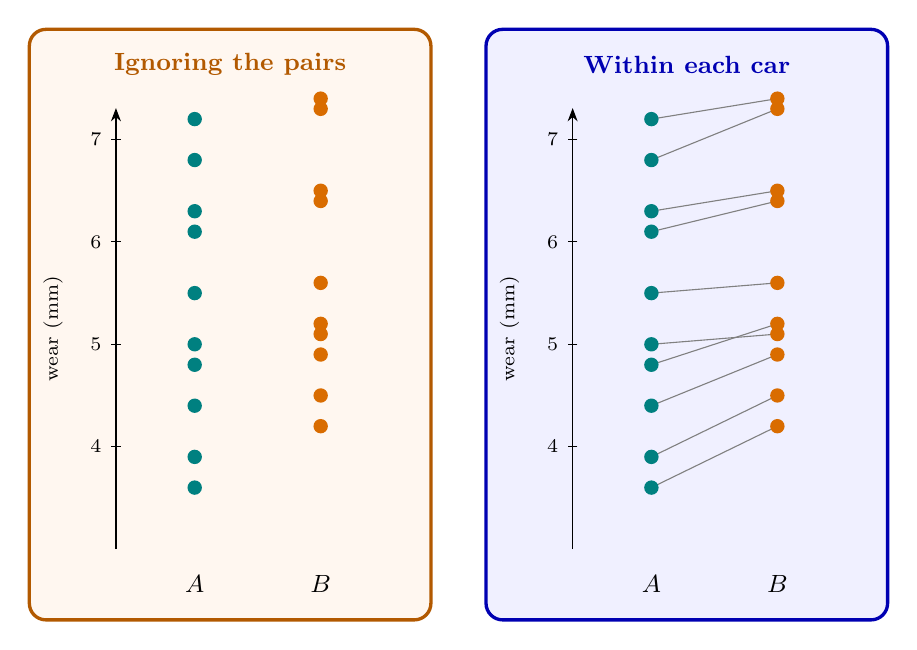
\begin{tikzpicture}
\begin{scope}[xshift=0cm]
\draw[rounded corners=6pt,very thick,draw=orange!70!black,fill=orange!6] (-1.1,-0.9) rectangle (4.0,6.6);
\node[font=\bfseries\small,orange!70!black] at (1.45,6.15) {Ignoring the pairs};
\draw[-Stealth] (0,0) -- (0,5.6);
\node[rotate=90,font=\scriptsize] at (-0.8,2.8) {wear (mm)};
\draw (0.06,1.3) -- (-0.06,1.3) node[left,font=\scriptsize] {4};
\draw (0.06,2.6) -- (-0.06,2.6) node[left,font=\scriptsize] {5};
\draw (0.06,3.9) -- (-0.06,3.9) node[left,font=\scriptsize] {6};
\draw (0.06,5.2) -- (-0.06,5.2) node[left,font=\scriptsize] {7};
\fill[teal] (1.0,2.34) circle (2.6pt);
\fill[orange!85!black] (2.6,2.86) circle (2.6pt);
\fill[teal] (1.0,4.03) circle (2.6pt);
\fill[orange!85!black] (2.6,4.42) circle (2.6pt);
\fill[teal] (1.0,1.17) circle (2.6pt);
\fill[orange!85!black] (2.6,1.95) circle (2.6pt);
\fill[teal] (1.0,5.46) circle (2.6pt);
\fill[orange!85!black] (2.6,5.72) circle (2.6pt);
\fill[teal] (1.0,3.25) circle (2.6pt);
\fill[orange!85!black] (2.6,3.38) circle (2.6pt);
\fill[teal] (1.0,1.82) circle (2.6pt);
\fill[orange!85!black] (2.6,2.47) circle (2.6pt);
\fill[teal] (1.0,4.94) circle (2.6pt);
\fill[orange!85!black] (2.6,5.59) circle (2.6pt);
\fill[teal] (1.0,2.6) circle (2.6pt);
\fill[orange!85!black] (2.6,2.73) circle (2.6pt);
\fill[teal] (1.0,0.78) circle (2.6pt);
\fill[orange!85!black] (2.6,1.56) circle (2.6pt);
\fill[teal] (1.0,4.29) circle (2.6pt);
\fill[orange!85!black] (2.6,4.55) circle (2.6pt);
\node[font=\small] at (1.0,-0.45) {$A$}; \node[font=\small] at (2.6,-0.45) {$B$};
\end{scope}
\begin{scope}[xshift=5.8cm]
\draw[rounded corners=6pt,very thick,draw=blue!70!black,fill=blue!6] (-1.1,-0.9) rectangle (4.0,6.6);
\node[font=\bfseries\small,blue!70!black] at (1.45,6.15) {Within each car};
\draw[-Stealth] (0,0) -- (0,5.6);
\node[rotate=90,font=\scriptsize] at (-0.8,2.8) {wear (mm)};
\draw (0.06,1.3) -- (-0.06,1.3) node[left,font=\scriptsize] {4};
\draw (0.06,2.6) -- (-0.06,2.6) node[left,font=\scriptsize] {5};
\draw (0.06,3.9) -- (-0.06,3.9) node[left,font=\scriptsize] {6};
\draw (0.06,5.2) -- (-0.06,5.2) node[left,font=\scriptsize] {7};
\draw[gray] (1.0,2.34) -- (2.6,2.86);
\fill[teal] (1.0,2.34) circle (2.6pt);
\fill[orange!85!black] (2.6,2.86) circle (2.6pt);
\draw[gray] (1.0,4.03) -- (2.6,4.42);
\fill[teal] (1.0,4.03) circle (2.6pt);
\fill[orange!85!black] (2.6,4.42) circle (2.6pt);
\draw[gray] (1.0,1.17) -- (2.6,1.95);
\fill[teal] (1.0,1.17) circle (2.6pt);
\fill[orange!85!black] (2.6,1.95) circle (2.6pt);
\draw[gray] (1.0,5.46) -- (2.6,5.72);
\fill[teal] (1.0,5.46) circle (2.6pt);
\fill[orange!85!black] (2.6,5.72) circle (2.6pt);
\draw[gray] (1.0,3.25) -- (2.6,3.38);
\fill[teal] (1.0,3.25) circle (2.6pt);
\fill[orange!85!black] (2.6,3.38) circle (2.6pt);
\draw[gray] (1.0,1.82) -- (2.6,2.47);
\fill[teal] (1.0,1.82) circle (2.6pt);
\fill[orange!85!black] (2.6,2.47) circle (2.6pt);
\draw[gray] (1.0,4.94) -- (2.6,5.59);
\fill[teal] (1.0,4.94) circle (2.6pt);
\fill[orange!85!black] (2.6,5.59) circle (2.6pt);
\draw[gray] (1.0,2.6) -- (2.6,2.73);
\fill[teal] (1.0,2.6) circle (2.6pt);
\fill[orange!85!black] (2.6,2.73) circle (2.6pt);
\draw[gray] (1.0,0.78) -- (2.6,1.56);
\fill[teal] (1.0,0.78) circle (2.6pt);
\fill[orange!85!black] (2.6,1.56) circle (2.6pt);
\draw[gray] (1.0,4.29) -- (2.6,4.55);
\fill[teal] (1.0,4.29) circle (2.6pt);
\fill[orange!85!black] (2.6,4.55) circle (2.6pt);
\node[font=\small] at (1.0,-0.45) {$A$}; \node[font=\small] at (2.6,-0.45) {$B$};
\end{scope}
\end{tikzpicture}
\caption{The tyre data. Between cars the wear ranges over nearly $4$ mm and swamps the brand difference (left). Joining the two tyres of each car
shows that every line rises: within a car, brand $B$ always wears more (right).}
\label{fig:pairs}
\end{figure}

The two analyses differ because the cars differ. The car-to-car variation is part of $s_p^2$ but cancels from every $d_j$, and the correlation between the
two tyres on a car is $0.989$. In general, if the two observations in a pair have common variance $\sigma_y^2$ and correlation $\rho$, then
\[
\Var(\bar d) = \frac{\Var(y_1 - y_2)}{n} = \frac{2\sigma_y^2(1 - \rho)}{n} ,
\]
against $2\sigma_y^2/n$ for two independent samples of size $n$. Pairing divides the variance by $1/(1 - \rho)$, here by about $90$.

\begin{remark}
Pairing is not free. The paired test has $n - 1$ degrees of freedom for error, the unpaired test $2n - 2$, so if the pairs are no more alike than units
chosen at random ($\rho \approx 0$), pairing wastes $n - 1$ degrees of freedom and gives a slightly less powerful test. The loss is small unless $n$ is very
small, and the potential gain is large, so when a natural pairing exists, it should be used. What is never acceptable is to choose between the
paired and unpaired analyses after seeing which gives the smaller $p$-value: the analysis must follow the design that was actually used.
\end{remark}

\subsection{Practice problems}

\begin{problem}
Two methods of making concrete blocks were compared, using independent random samples of blocks. Method $1$ gave
$n_1 = 12$ blocks with $\bar y_1 = 48.2$ and $s_1 = 3.1$; method $2$ gave $n_2 = 10$ blocks with $\bar y_2 = 45.1$ and $s_2 = 2.6$. Test whether the mean compressive strengths
differ at $\alpha = 0.05$, and give a $95\%$ confidence interval for $\mu_1 - \mu_2$.
\end{problem}

\begin{solution}
The pooled variance is
\[
s_p^2 = \frac{11(3.1)^2 + 9(2.6)^2}{20} = \frac{105.71 + 60.84}{20} = 8.3275 , \qquad s_p = 2.886 ,
\]
and the standard error is $2.886\sqrt{1/12 + 1/10} = 1.2356$. Then $t_0 = (48.2 - 45.1)/1.2356 = 2.509$. Since $t_{0.025,20} = 2.086$, $H_0$ is rejected
($p = 0.021$). The $95\%$ interval is $3.1 \pm 2.086(1.2356)$, that is $(0.52,\ 5.68)$.
\end{solution}

\begin{problem}
Show that $S_p^2$ is an unbiased estimator of $\sigma^2$, and that when $n_1 = n_2$ the Welch statistic $t_0^*$ equals the pooled statistic $t_0$.
\end{problem}

\begin{solution}
$E(S_i^2) = \sigma^2$ for each sample, so $E(S_p^2) = [(n_1 - 1)\sigma^2 + (n_2 - 1)\sigma^2]/(n_1 + n_2 - 2) = \sigma^2$. If $n_1 = n_2 = n$, then $S_p^2 = (S_1^2 + S_2^2)/2$, and
\[
S_p^2\Bigl(\frac1n + \frac1n\Bigr) = \frac{S_1^2 + S_2^2}{n} = \frac{S_1^2}{n} + \frac{S_2^2}{n} ,
\]
so the two denominators are equal and $t_0^* = t_0$. Only the reference distribution differs: $t_{2n-2}$ for the pooled test, $t_\nu$ with $\nu \le 2n - 2$ for
Welch's.
\end{solution}

\begin{problem}
Show that Welch's degrees of freedom satisfy $\min(n_1, n_2) - 1 \le \nu \le n_1 + n_2 - 2$.
\end{problem}

\begin{solution}
Write $u_i = s_i^2/n_i > 0$ and $f_i = n_i - 1$, so $\nu = (u_1 + u_2)^2/(u_1^2/f_1 + u_2^2/f_2)$. For the lower bound, with $f = \min(f_1, f_2)$,
\[
\frac{u_1^2}{f_1} + \frac{u_2^2}{f_2} \le \frac{u_1^2 + u_2^2}{f} \le \frac{(u_1 + u_2)^2}{f} ,
\]
so $\nu \ge f$. For the upper bound, by the Cauchy--Schwarz inequality,
\[
(u_1 + u_2)^2 = \Bigl(\frac{u_1}{\sqrt{f_1}}\sqrt{f_1} + \frac{u_2}{\sqrt{f_2}}\sqrt{f_2}\Bigr)^2 \le \Bigl(\frac{u_1^2}{f_1} + \frac{u_2^2}{f_2}\Bigr)(f_1 + f_2) ,
\]
so $\nu \le f_1 + f_2 = n_1 + n_2 - 2$, with equality when $u_1/f_1 = u_2/f_2$.
\end{solution}

\begin{problem}
An experimenter expects $\sigma \approx 5$ and wants power $0.80$ to detect a difference of $4$ units between two treatment means, using a two-sided test at
$\alpha = 0.05$. Find the number of replicates per treatment from the normal approximation, and comment on the exact answer.
\end{problem}

\begin{solution}
With $z_{0.025} = 1.960$ and $z_{0.20} = 0.842$,
\[
n = \frac{2(1.960 + 0.842)^2(25)}{16} = 24.53 ,
\]
so $25$ per treatment. The exact power from the non-central $t$ distribution is $0.791$ with $n = 25$ and $0.807$ with $n = 26$, so $26$ are required. As in the
text, the approximation falls short by about one replicate, because it treats $\sigma$ as known.
\end{solution}

\begin{problem}
The systolic blood pressure of six patients was measured before and after a month on a new drug:
\begin{center}
\begin{tabular}{l|cccccc}
patient & 1 & 2 & 3 & 4 & 5 & 6 \\
\hline
before & $142$ & $150$ & $138$ & $161$ & $147$ & $155$ \\
after & $136$ & $144$ & $139$ & $150$ & $141$ & $149$
\end{tabular}
\end{center}
Test whether the drug changes mean blood pressure, and give a $95\%$ confidence interval for the mean reduction. What does this design not control?
\end{problem}

\begin{solution}
The reductions are $d = (6, 6, -1, 11, 6, 6)$, with $\bar d = 5.667$ and $s_d = 3.830$. Then
\[
t_0 = \frac{5.667}{3.830/\sqrt6} = 3.624 ,
\]
against $t_{0.025,5} = 2.571$, so $H_0$ is rejected ($p = 0.015$). The interval is $5.667 \pm 2.571(1.5635)$, that is $(1.65,\ 9.69)$.

Each patient is a block, but the two ``treatments'' (before and after) cannot be randomised in order: after always follows before. Any change
over the month, such as the season, the attention of being in a study, or regression towards the mean in patients selected for high
pressure, is confounded with the drug. A control group taking a placebo, with patients allocated at random, would be needed to separate
them.
\end{solution}

\begin{problem}
In a paired design the two observations in a pair have variance $\sigma_y^2$ and correlation $\rho$. For what values of $\rho$ does pairing give a smaller variance
for the estimated difference than two independent samples of the same size? Explain why the comparison of the two tests also involves the
degrees of freedom.
\end{problem}

\begin{solution}
The variances are $2\sigma_y^2(1 - \rho)/n$ and $2\sigma_y^2/n$, so pairing is better exactly when $\rho > 0$; when units within a pair are negatively correlated it
is worse. But the tests also differ in their error degrees of freedom, $n - 1$ against $2n - 2$, and so in the critical value $t_{\alpha/2}$. For small $n$ and small
positive $\rho$ the larger critical value of the paired test can outweigh its smaller variance. In practice pairs are formed because their members
are alike, $\rho$ is substantial, and the variance reduction dominates.
\end{solution}

\section*{References}
\addcontentsline{toc}{section}{References}

\subhead{Prescribed texts}
\begin{enumerate}
\item Montgomery, D. C. (2001), \emph{Design and Analysis of Experiments} (5th ed.), New York, Wiley.
\item Oehlert, G. W. (2000), \emph{A First Course in Design and Analysis of Experiments}, New York, W. H. Freeman.
\end{enumerate}

\subhead{Recommended texts}
\begin{enumerate}
\item Mason, R. L., Gunst, R. F., and Hess, J. L. (2003), \emph{Statistical Design and Analysis of Experiments} (2nd ed.), New York, Wiley.
\item John, P. W. M. (1998), \emph{Statistical Design and Analysis of Experiments}, Philadelphia, Society for Industrial and Applied Mathematics.
\end{enumerate}

\subhead{Further reading}
\begin{enumerate}
\item Box, G. E. P., Hunter, J. S., and Hunter, W. G. (2005), \emph{Statistics for Experimenters} (2nd ed.), Hoboken, NJ, Wiley.
\item Cox, D. R. (1958), \emph{Planning of Experiments}, New York, Wiley.
\item Fisher, R. A. (1935), \emph{The Design of Experiments}, Edinburgh, Oliver and Boyd.
\end{enumerate}

\end{document}
